\documentclass[12pt]{jarticle}
\usepackage{TUSIreport}
\usepackage{otf}
\usepackage[dvipdfmx]{graphicx}
\usepackage[dvipdfmx]{color}
\usepackage{amsmath}
\usepackage{amssymb}
\usepackage{color}
\usepackage{hhline}
\usepackage{fancybox,ascmac}
\usepackage{multirow}
\usepackage{url}
\usepackage{bm}
\usepackage{listings,jlisting}
%%%%%%%%%%%%%%%%%%
\lstdefinestyle{py}{
    language={Python},
    backgroundcolor={\color[gray]{.85}},
    basicstyle={\small},
    identifierstyle={\small},
    commentstyle={\small\ttfamily \color[rgb]{0,0.5,0}},
    keywordstyle={\small\bfseries \color[rgb]{1,0,0}},
    ndkeywordstyle={\small},
    stringstyle={\small\ttfamily \color[rgb]{0,0,1}},
    frame={tb},
    breaklines=true,
    columns=[l]{fullflexible},
    xrightmargin=0zw,
    xleftmargin=3zw,
    numberstyle={\scriptsize},
    stepnumber=1,
    numbersep=1zw,
    morecomment=[l]{//}
}
\begin{document}
%%%%%%%%%%%%%%%%%%%%%%%%%%%%%%%%%%%%%%%%%%%%%%%%%%%%%%%%
% 表紙を出力する場合は,\提出者と\共同実験者をいれる
% \提出者{科目名}{課題名}{提出年}{提出月}{提出日}{学籍番号}{氏名}
% \共同実験者{一人目}{二人目}{..}{..}{..}{..}{..}{八人目}
%%%%%%%%%%%%%%%%%%%%%%%%%%%%%%%%%%%%%%%%%%%%%%%%%%%%%%%
\提出者{情報工学実験3}{課題2 パターン認識}
{2021}{6}{10}{4619055}{辰川力駆}
%%%%%%%%%%%%%%%%%%%%%%%%%%%%%%%%%%%%%%%%%%%%%%%%%%%%%%%%%
\共同実験者{}{}{}{}{}{}{}{}
%%%%%%%%%%%%%%%%%%%%%%%%%%%%%%%%%%%%%%%%%%%%%%%%%%%%%%%%%
% 表紙を出力する場合はコメントアウトしない
%%%%%%%%%%%%%%%%%%%%%%%%%%%%%%%%%%%%%%%%%%%%%%%%%%%%%%%%%
\表紙出力
%%%%%%%%%%%%%%%%%%%%%%%%%%%%%%%%%%%%%%%%%%%%%%%%%%%%%%%
% 以下はレポート本体,reportmain.tex に書いてある.
% \inputを使っているが,直接書いても良い.
%%%%%%%%%%%%%%%%%%%%%%%%%%%%%%%%%%%%%%%%%%%%%%%%%%%%%%%
\section{はじめに}
パターン認識とは、
入力データをあらかじめ定めていた複数のクラスの1つに対応させる処理のことをいう。
分類を行うクラスの種類に応じて、パターン認識は大きく、
「分類問題」と「予測問題」に分けることができる。
また、分類問題、予測問題の両方に関して、
「教師あり学習」と「教師なし学習」の2つが存在しており、
本実験では、入力データと出力の組みが与えられているデータを利用したパターン認識である
「教師あり学習」について理解する。


\section{授業内課題}
\subsection{課題内容}
\begin{itemize}
    \item [(1)]配布した「pima\_tr.csv」と「pima\_te.csv」を読み込み、
          2つのデータを縦方向に結合し、その後1列目を削除する。
          また、結合したデータのtype以外の列を標準化する。
    \item [(2)]$k$近傍法において、$k=3$に固定し、このときの訓練データに対するTrue Positive Rateを求める。
          また、テストデータに対するTrue Positive Rateも求める。
\end{itemize}
\subsection{手順}
\begin{enumerate}
    \item Jupiter Notebook上でPythonのプログラムを作成する。
    \item 作成したソースコードを実行する。
\end{enumerate}
\subsection{結果}
作成したソースコードは付録のソースコード1と2に載せた。
ソースコード2を実行した結果、
$k$近傍法において、$k=3$に固定したときの訓練データに対するTrue Positive Rateは、

\begin{eqnarray}
    \text{True Positive Rate}&=& 0.75 \nonumber
\end{eqnarray}

また、テストデータに対するTrue Positive Rateは、

\begin{eqnarray}
    \text{True Positive Rate}&=& 0.484848 \nonumber
\end{eqnarray}
となった。

\clearpage

\subsection{考察}
訓練データとテストデータのTrue Positive Rateを比較すると、
訓練データの方が高かった。
これは、偶然なったわけではなく必然である。
理由は、訓練データを学習させたあとに、
訓練データとテストデータのTrue Positive Rateを求めたからである。

訓練データを学習させた後に
テストデータのTrue Positive Rateがどうなっているかを見ると、$0.484848$
であった。
つまり、糖尿病を判断できるのはほぼ半分であると分かる。
逆に言えば糖尿病なのに糖尿病と判定されない人が半分もいることになる。
したがって、この学習モデルを用いるのは適切でないと考える。

\section{レポート課題}
\subsection{課題内容}
\begin{itemize}
    \item [(1)]2クラス分類問題の場合、評価指標として混同行列が使われるが、
          多クラス分類の際の評価指標について調べ、まとめる。
    \item [(2)]True Positive Rateを高めることを目標にして、
          訓練データとテストデータにStratifiedになるように8:2の割合で分割する。
          さらに、$k$近傍法を用いて、
          分割した訓練データに対して交差検証を行い最適な$k$の値を求め、
          テストデータに対する正解率を予測し、
          その時のTrue Positive Rateを求める。
\end{itemize}
\subsection{手順}
\begin{itemize}
    \item [(1)]検索をして、文献を探す。
    \item [(2)]\begin{enumerate}
              \item Jupiter Notebook上でPythonのプログラムを作成する。
              \item 作成したソースコードを実行する。
          \end{enumerate}
\end{itemize}

\subsection{結果}
\subsubsection*{(1)}
多クラス分類の際も、最初は同じように混同行列作成する。
計算するときは、クラス分のTrue PositiveやFalse Positiveなどを作成する。
2つのクラスと同様に正しく判定されたものはTrue Positiveとして、
それ以外はすべてFalse Positiveとする。

多クラス分類の特別な評価指標として、マクロ平均とマイクロ平均がある。
マクロ平均は各クラスの評価指標の平均を計算しているため、
各クラスの平均の評価指標を表している。
各クラスにサンプル数に偏りがあっても、各クラスが公平に扱われる。
たとえば、マクロ平均適合率は、クラス$L_i$の適合率を$P_i$とすると、
\begin{eqnarray}
    \text{マクロ平均適合率}=\frac{\Sigma^N_{i=1} P_i}{N} \nonumber
\end{eqnarray}
と表される。

マイクロ平均はデータ全体を考慮して計算される指標であり、
データセット全体に対する平等的な評価指標といえる。
しかし、各クラスのサンプルの数に偏りが大きい場合、
サンプル数の大きいクラスの性能が全体の性能を代表してしまう可能性がある。
たとえば、マイクロ平均適合率は、クラス$L_i$のTrue Positiveを$TP_i$として、
False Positiveを$FP_i$とすると、
\begin{eqnarray}
    \text{マイクロ平均適合率}=\frac{\Sigma^N_{i=1} TP_i}{\Sigma^N_{i=1} (TP_i+FP_i)} \nonumber
\end{eqnarray}
と表される。

\subsubsection*{(2)}
作成したソースコードは付録のソースコード3に載せた。
実行した結果は、交差検証したときのグラフとその中で最適な$k$の値を表示し、
その$k$の値の時のテストデータに対するAccuracy ScoreとTrue Positive Rateを表示した。

図1は、交差検証したときのMSEの大きさを見るグラフである。
\begin{figure}[h]
    \begin{center}
        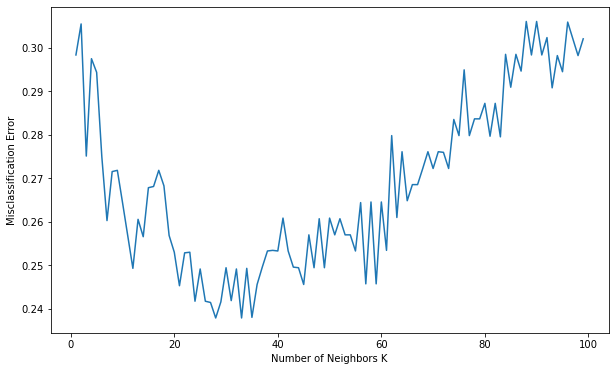
\includegraphics[scale=0.6]{kadai2_2_1.png}
    \end{center}
    \caption{交差検証のグラフ}
\end{figure}

交差検証より、最適な$k$の値は$k=33$と分かった。
また、$k=33$の時のテストデータに対するAccuracy ScoreとTrue Positive Rateは、
\begin{eqnarray}
    \text{Accuracy Score}&=& 0.835821 \nonumber \\
    \text{True Positive Rate}&=& 0.545455 \nonumber
\end{eqnarray}
となった。

\subsection{考察}
授業内課題で作成した学習モデルと比較すると、True Positive Rateの値が高くなっていることが分かる。
これは最適な$k=33$に変更したことにより良くなっているということである。

\section{感想}
今回の講義動画に関しては、実際にコードを実行しながら説明をしていたので分かりやすかった。
改善はあまりしなくていいと考えるが、
あえて言うならば、好みがわかれるが自分的には動画を1つにまとめてくれる方が見やすかった。

\begin{thebibliography}{99}
    \label{sannkoubunnkenn_chapter}
    \bibitem[1]{a}
    多クラス分類の性能指標

    \url{https://kunsen.net/2021/03/18/post-3653/#i-2}

    最終閲覧日2021/06/12

    \bibitem[2]{b}
    多クラスの評価指標 | 多クラス予測モデルを評価するときに指標のマクロ平均あるいはマイクロ平均を使う

    \url{https://axa.biopapyrus.jp/machine-learning/model-evaluation/multiclass-evaluation.html}

    最終閲覧日2021/06/12
\end{thebibliography}

\clearpage
\appendix
\section{付録}
\begin{lstlisting}[style = py,caption=授業内課題(1)]
    import pandas as pd
    from sklearn import preprocessing
    pima_train = pd.read_csv('data/pima_tr.csv',encoding='UTF-8')
    pima_test = pd.read_csv('data/pima_te.csv',encoding='UTF-8')
    
    group_data = pd.concat([pima_train, pima_test], ignore_index=True)
    del group_data['Unnamed: 0']
    X = preprocessing.scale(group_data[['npreg','glu','bp','skin','bmi','ped','age']])
\end{lstlisting}


\begin{lstlisting}[style = py,caption=授業内課題(2)]
    import pandas as pd
    from sklearn import preprocessing
    from sklearn.model_selection import train_test_split
    from sklearn.metrics import confusion_matrix
    from sklearn.neighbors import KNeighborsClassifier
    pima_train = pd.read_csv('data/pima_tr.csv',encoding='UTF-8')
    pima_test = pd.read_csv('data/pima_te.csv',encoding='UTF-8')
    
    group_data = pd.concat([pima_train, pima_test], ignore_index=True)
    del group_data['Unnamed: 0']
    
    X = preprocessing.scale(group_data[['npreg','glu','bp','skin','bmi','ped','age']])
    y = group_data.type
    
    X_train, X_test, y_train, y_test = train_test_split(X, y, random_state=0, train_size=0.7, stratify=y)
    
    knn = KNeighborsClassifier(n_neighbors = 3)
    knn.fit(X_train, y_train)
    
    y_pred = knn.predict(X_train)
    cmat = confusion_matrix(y_train, y_pred, labels=['Yes', 'No'])
    TP, FN = cmat[0, 0], cmat[0, 1]
    print('訓練データに対するTrue Positive Rate:',TP/(TP+FN))
    
    y_pred = knn.predict(X_test)
    cmat = confusion_matrix(y_test, y_pred, labels=['Yes', 'No'])
    TP, FN = cmat[0, 0], cmat[0, 1]
    print('テストデータに対するTrue Positive Rate:',TP/(TP+FN))
\end{lstlisting}

\begin{lstlisting}[style = py,caption=レポート課題(2)]
    import numpy as np
    import pandas as pd
    from sklearn import preprocessing
    from sklearn.model_selection import train_test_split
    from sklearn.metrics import confusion_matrix
    from sklearn.neighbors import KNeighborsClassifier
    from sklearn.metrics import accuracy_score
    from sklearn.model_selection import cross_val_score
    import matplotlib.pyplot as plt
    %matplotlib inline
    pima_train = pd.read_csv('data/pima_tr.csv',encoding='UTF-8')
    pima_test = pd.read_csv('data/pima_te.csv',encoding='UTF-8')
    
    group_data = pd.concat([pima_train, pima_test], ignore_index=True)
    del group_data['Unnamed: 0']
    
    X = preprocessing.scale(group_data[['npreg','glu','bp','skin','bmi','ped','age']])
    y = group_data.type
    
    X_train, X_test, y_train, y_test = train_test_split(X, y, random_state=0, train_size=0.8, stratify=y)
    
    neighbors = list(range(1, 100))
    cv_scores = []
    for k in neighbors:
        knn = KNeighborsClassifier(n_neighbors = k)
        scores = cross_val_score(
            knn,
            X_train,
            y_train,
            cv = 10,
            scoring = 'accuracy',
            n_jobs = -1
        )
        cv_scores.append(np.mean(scores))
    
    MSE = [1 - x for x in cv_scores]
    
    optimal_k = neighbors[MSE.index(min(MSE))]
    print('The optimal number of k is %d' % optimal_k)
    
    fig, ax = plt.subplots(figsize = (10, 6))
    ax.plot(neighbors, MSE)
    ax.set_xlabel('Number of Neighbors K')
    ax.set_ylabel('Misclassification Error')
    
    knn = KNeighborsClassifier(n_neighbors = optimal_k)
    knn.fit(X_train, y_train)
    
    y_pred = knn.predict(X_test)
    cmat = confusion_matrix(y_test, y_pred, labels=['Yes', 'No'])
    TP, FN = cmat[0, 0], cmat[0, 1]
    print('テストデータに対するTrue Positive Rate:',TP/(TP+FN))
    
    print('テストデータに対するAccuracy Score:',accuracy_score(y_test, y_pred))
\end{lstlisting}


%%%%%%%%%%%%%%%%%%%%%%%%%%%%%%%%%%%%%%%%%%%%%%%%%%%%%%%
\end{document}